%{{第一回}}{第一回}}

\chapter{甄士隐梦幻识通灵 贾雨村风尘怀闺秀}\label{calibre_pb_0}

  {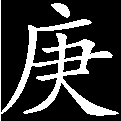
\includegraphics[width=3mm]{../Images/00004}此开卷第一回也。作者自云:因曾历过一番梦幻之后,故将真事隐去,而借通灵之说,撰此《石头记》一书也,故曰``甄士隐''云云。但书中所记何事何人?自又云:``今风尘碌碌,一事无成,忽念及当日所有之女子,一一细考较去,觉其行止见识皆出于我之上。何我堂堂须眉,诚不若此裙钗哉?{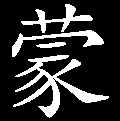
\includegraphics[width=3mm]{../Images/00006}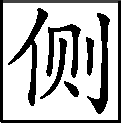
\includegraphics[width=3mm]{../Images/00011}\footnotesize  何非梦幻,何不通灵?作者托言,原当有自。受气清浊,本无男女{[}之{]}别。}实愧则有馀,悔又无益之大无可如何之日也!当此,则自欲将已往所赖天恩祖德,锦衣纨绔之时,饫甘餍肥之日,背父兄教育之恩,负师友规谈之德,以至今日一技无成、半生潦倒之罪,{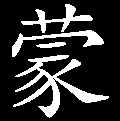
\includegraphics[width=3mm]{../Images/00006}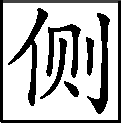
\includegraphics[width=3mm]{../Images/00011}\footnotesize 明告看者。}编述一集,以告天下人:我之罪固不免,然闺阁中本自历历有人,万不可因我之不肖,自护己短,一并使其泯灭也。{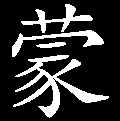
\includegraphics[width=3mm]{../Images/00006}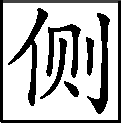
\includegraphics[width=3mm]{../Images/00011}\footnotesize 因为传他,并可传我。}虽今日之茅椽蓬牖,瓦灶绳床,其晨夕风露,阶柳庭花,亦未有妨我之襟怀笔墨。虽我未学,下笔无文,又何妨用假语村言敷演出一段故事来?亦可使闺阁昭传,复可悦世之目,破人愁闷,不亦宜乎?''故曰``贾雨村''云云。}

  {此回中凡用``梦''用``幻''等字,是提醒阅者眼目,亦是此书立意本旨。}
列位看官,你道此书从何而来?\footnote{底本正文从此开始。按:本书第一至八回、第十三至十六回、第二十五至二十八回以甲戌本为底本,第六十四回、第六十七回以列藏本为底本,其馀部分以庚辰本为底本,下文所称底本均以此为据,不另注。}{\textsuperscript{②}\label{lnkback_2_a}}说起根由虽近荒唐,{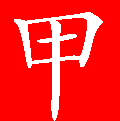
\includegraphics[width=3mm]{../Images/00002}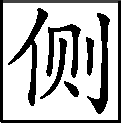
\includegraphics[width=3mm]{../Images/00011}\footnotesize 自占地步。◇自首荒唐,妙!}细谙则深有趣味。待在下将此来历注明,方使阅者了然不惑。

原来,女娲氏炼石补天之时,{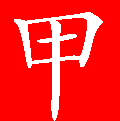
\includegraphics[width=3mm]{../Images/00002}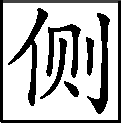
\includegraphics[width=3mm]{../Images/00011} \footnotesize \kaishu 补天济世,勿认真用常言。}于大荒山{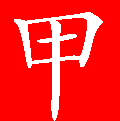
\includegraphics[width=3mm]{../Images/00002}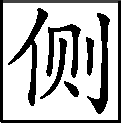
\includegraphics[width=3mm]{../Images/00011}\footnotesize 荒唐也。}无稽崖{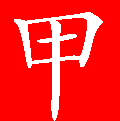
\includegraphics[width=3mm]{../Images/00002}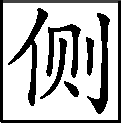
\includegraphics[width=3mm]{../Images/00011}\footnotesize 无稽也。}炼成高经十二丈、{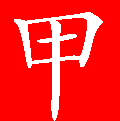
\includegraphics[width=3mm]{../Images/00002}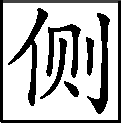
\includegraphics[width=3mm]{../Images/00011}\footnotesize 总应十二钗。}方经二十四丈{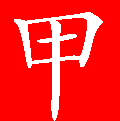
\includegraphics[width=3mm]{../Images/00002}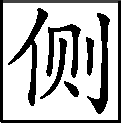
\includegraphics[width=3mm]{../Images/00011}\footnotesize 照应副十二钗。}顽石三万六千五百零一块。娲皇氏只用了三万六千五百块,{{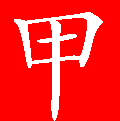
\includegraphics[width=3mm]{../Images/00002}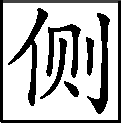
\includegraphics[width=3mm]{../Images/00011}\footnotesize 合周天之数。 }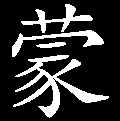
\includegraphics[width=3mm]{../Images/00006}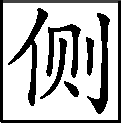
\includegraphics[width=3mm]{../Images/00011}\footnotesize 数足,偏遗我。``不堪入选''句中透出心眼。}只单单的剩了一块未用,{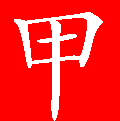
\includegraphics[width=3mm]{../Images/00002}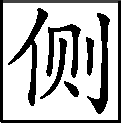
\includegraphics[width=3mm]{../Images/00011}\footnotesize 剩了这一块便生出这许多故事。使当日虽不以此补天,就该去补地之坑陷,使地平坦,而不得有此一部鬼话。}便弃在此山青埂峰下。{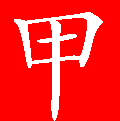
\includegraphics[width=3mm]{../Images/00002}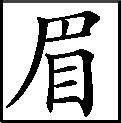
\includegraphics[width=3mm]{../Images/00010}\footnotesize  妙!自谓落堕情根,故无补天之用。}谁知此石自经煅炼之后,灵性已通,{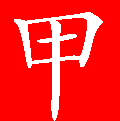
\includegraphics[width=3mm]{../Images/00002}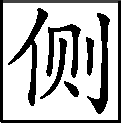
\includegraphics[width=3mm]{../Images/00011}\footnotesize 煅炼后性方通。甚哉,人生不能学也!}因见众石俱得补天,独自己无材不堪入选,遂自怨自叹,日夜悲号惭愧。

一日,正当嗟悼之际,俄见一僧一道远远而来,生得骨格不凡,丰神迥别,{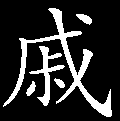
\includegraphics[width=3mm]{../Images/00005} 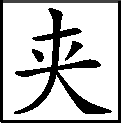
\includegraphics[width=3mm]{../Images/00012}\footnotesize   这是真像,非幻像也。}说说笑笑来至峰下,坐于石边,高谈快论。先是说些云山雾海、神仙玄幻之事,后便说到红尘中荣华富贵。此石听了,不觉打动凡心,也想要到人间去享一享这荣华富贵,但自恨粗蠢,不得已,便口吐人言,{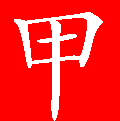
\includegraphics[width=3mm]{../Images/00002}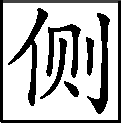
\includegraphics[width=3mm]{../Images/00011}\footnotesize 竟有人问:``口生于何处?''其无心肝,可笑可恨之极!}向那僧道说道:``大师,弟子蠢物,{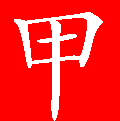
\includegraphics[width=3mm]{../Images/00002}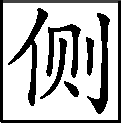
\includegraphics[width=3mm]{../Images/00011}\footnotesize 岂敢岂敢。}不能见礼了。适闻二位谈那人世间荣耀繁华,心切慕之。弟子质虽粗蠢,{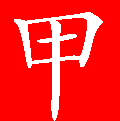
\includegraphics[width=3mm]{../Images/00002}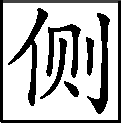
\includegraphics[width=3mm]{../Images/00011}\footnotesize 岂敢岂敢。}性却稍通,况见二师仙形道体,定非凡品,必有补天济世之材,利物济人之德。如蒙发一点慈心,携带弟子得入红尘,在那富贵场中、温柔乡里受享几年,自当永佩洪恩,万劫不忘也。''二仙师听毕,齐憨笑道:``善哉,善哉!那红尘中有却有些乐事,但不能永远依恃,况又有`美中不足,好事多魔'八个字紧相连属,瞬息间则又乐极悲生、人非物换,究竟是到头一梦、万境归空。{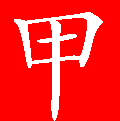
\includegraphics[width=3mm]{../Images/00002}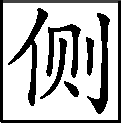
\includegraphics[width=3mm]{../Images/00011}\footnotesize 四句乃一部之总纲。}倒不如不去的好。''

这石凡心已炽,那里听得进这话去,乃复苦求再四。二仙知不可强制,乃叹道:``此亦静极思动,无中生有之数也。既如此,我们便携你去受享受享,只是到不得意时,切莫后悔。''石道:``自然,自然。''那僧又道:``若说你性灵,却又如此质蠢,并更无奇贵之处,如此也只好踮脚而已。{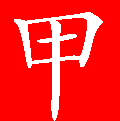
\includegraphics[width=3mm]{../Images/00002}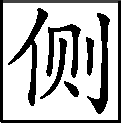
\includegraphics[width=3mm]{../Images/00011}\footnotesize 煅炼过尚与人踮脚,不学者又当如何?}也罢,我如今大施佛法助你{[}一{]}助,待劫终之日,复还本质,以了此案。{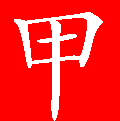
\includegraphics[width=3mm]{../Images/00002}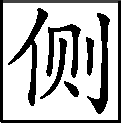
\includegraphics[width=3mm]{../Images/00011}\footnotesize 妙!佛法亦须偿还,况世人之债乎?近之赖债者来看此句。所谓游戏笔墨也。}你道好否?''石头听了,感谢不尽。那僧便念咒书符,大展幻{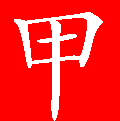
\includegraphics[width=3mm]{../Images/00002}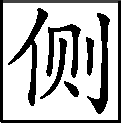
\includegraphics[width=3mm]{../Images/00011}\footnotesize 明点``幻''字。好!}术,将一块大石登时变成{[}\^{}③\^{}{]}(../Text/part0005\_split\_000.html\#lnkback\_3\_a)\{\#navto\_3\_a\}\elegantpar{一块鲜明莹洁的美玉,且又缩成扇坠大小的可佩可拿。}{脚注还没转换成功,标题没有在章字处换行也难受,标题显得长了,应该换一下行比较好}{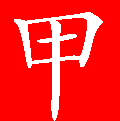
\includegraphics[width=3mm]{../Images/00002}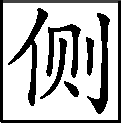
\includegraphics[width=3mm]{../Images/00011}\footnotesize 奇诡险怪之文,有如髯苏《石钟》《赤壁》用幻处。}那僧托于掌上,笑道:``形体倒也是个宝物了!{{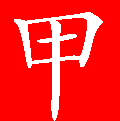
\includegraphics[width=3mm]{../Images/00002}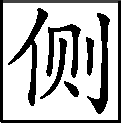
\includegraphics[width=3mm]{../Images/00011}\footnotesize 自愧之语。 }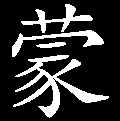
\includegraphics[width=3mm]{../Images/00006}\includegraphics[width=3mm]{../Images/00011}\footnotesize 世上人原自据看得见处为凭。}还只没有实在的好处,{\includegraphics[width=3mm]{../Images/00002}\includegraphics[width=3mm]{../Images/00011}\footnotesize 妙极!今之金玉其外败絮其中者,见此大不欢喜。}须得再镌上数字,使人一见便知是奇物方妙。{\includegraphics[width=3mm]{../Images/00002}\includegraphics[width=3mm]{../Images/00011}\footnotesize 世上原宜假,不宜真也。◇谚云:``一日卖了三千假,三日卖不出一个真。''信哉!}然后好携你到那昌明隆盛之邦,{\includegraphics[width=3mm]{../Images/00002}\includegraphics[width=3mm]{../Images/00011}\footnotesize 伏长安大都。}诗礼簪缨之族,{\includegraphics[width=3mm]{../Images/00002}\includegraphics[width=3mm]{../Images/00011}\footnotesize 伏荣国府。}花柳繁华地,{\includegraphics[width=3mm]{../Images/00002}\includegraphics[width=3mm]{../Images/00011}\footnotesize 伏大观园。}温柔富贵乡{\includegraphics[width=3mm]{../Images/00002}\includegraphics[width=3mm]{../Images/00011}\footnotesize 伏紫芸轩。}去安身乐业。''{\includegraphics[width=3mm]{../Images/00002}\includegraphics[width=3mm]{../Images/00011}\footnotesize 何不再添一句云``择个绝世情痴作主人''?}石头听了,喜不能禁,乃问:``不知赐了弟子那几件奇处,{\includegraphics[width=3mm]{../Images/00002}\includegraphics[width=3mm]{../Images/00011}\footnotesize 可知若果有奇贵之处,自己亦不知者。若自以奇贵而居,究竟是无真奇贵之人。}又不知携了弟子到何地方?{\includegraphics[width=3mm]{../Images/00002} \includegraphics[width=3mm]{../Images/00010}\footnotesize 昔子房后谒黄石公,惟见一石。子房当时恨不随此石去。余亦恨不能随此石而去也。聊供阅者一笑。}望乞明示,使弟子不惑。''那僧笑道:``你且莫问,日后自然明白的。''说着,便袖了这石,同那道人飘然而去,竟不知投奔何方何舍。

后来,又不知过了几世几劫,因有个空空道人访道求仙,忽从这大荒山无稽崖青埂峰下经过,忽见一大石上字迹分明,编述历历。空空道人乃从头一看,原来就是无材补天、幻形入世,{\includegraphics[width=3mm]{../Images/00002}\includegraphics[width=3mm]{../Images/00011}\footnotesize 八字便是作者一生惭恨。}蒙茫茫大士、渺渺真人携入红尘,历尽离合悲欢、炎凉世态的一段故事。后面又有一首偈云:

  无材可去补苍天,{\includegraphics[width=3mm]{../Images/00002}\includegraphics[width=3mm]{../Images/00011}\footnotesize 书之本旨。}枉入红尘若许年。{\includegraphics[width=3mm]{../Images/00002}\includegraphics[width=3mm]{../Images/00011}\footnotesize 惭愧之言,呜咽如闻。}

  此系身前身后事,倩谁记去作奇传?

诗后便是此石堕落之乡,投胎之处,亲自经历的一段陈迹故事。其中家庭闺阁琐事,以及闲情诗词倒还全备,或{\includegraphics[width=3mm]{../Images/00002}\includegraphics[width=3mm]{../Images/00011}\footnotesize ``或''字谦得好。}可适趣解闷,然朝代年纪,地舆邦国,{\includegraphics[width=3mm]{../Images/00002}\includegraphics[width=3mm]{../Images/00011}\footnotesize 若用此套者,胸中必无好文字,手中断无新笔墨。}却反失落无考。{{\includegraphics[width=3mm]{../Images/00002}\includegraphics[width=3mm]{../Images/00011}\footnotesize 据余说,却大有考证。 }\includegraphics[width=3mm]{../Images/00006}\includegraphics[width=3mm]{../Images/00011}\footnotesize 妙在``无考''。}

空空道人遂向石头说道:``石兄,你这一段故事,据你自己说有些趣味,故编写在此,意欲问世传奇。据我看来:第一件,无朝代年纪可考,{\includegraphics[width=3mm]{../Images/00002}\includegraphics[width=3mm]{../Images/00011}\footnotesize 先驳得妙。}第二件,并无大贤大忠理朝廷、治风俗的善政,{\includegraphics[width=3mm]{../Images/00002}\includegraphics[width=3mm]{../Images/00011}\footnotesize 将世人欲驳之腐言,预先代人驳尽。妙!}其中只不过几个异样的女子,或情或痴,或小才微善,亦无班姑、蔡女之德能。我纵抄去,恐世人不爱看呢。''

石头笑答道:``我师何太痴耶!若云无朝代可考,今我师竟假借汉唐等年纪添缀,又有何难?{\includegraphics[width=3mm]{../Images/00002}\includegraphics[width=3mm]{../Images/00011}\footnotesize 所以答得好。}但我想,历来野史,皆蹈一辙,莫如我这不借此套者,反倒新奇别致,不过只取其事体情理罢了,又何必拘拘于朝代年纪哉!再者,市井俗人喜看理治之书者甚少,爱看适趣闲文者特多。历来野史,或讪谤君相,或贬人妻女,{\includegraphics[width=3mm]{../Images/00002}\includegraphics[width=3mm]{../Images/00011}\footnotesize 先批其大端。}奸淫凶恶,不可胜数。更有一种风月笔墨,其淫秽污臭,涂毒笔墨,坏人子弟,又不可胜数。至若佳人才子等书,则又千部共出一套,且其中终不能不涉于淫滥,以致满纸潘安子建、西子文君,不过作者要写出自己的那两首情诗艳赋来,故假拟出男女二人名姓,又必旁出一小人其间拨乱,{\includegraphics[width=3mm]{../Images/00006}\includegraphics[width=3mm]{../Images/00011}\footnotesize 放笔以情趣世人,并评倒多少传奇。文气淋漓,字句切实。}亦如剧中之小丑然。且鬟婢开口即者也之乎,非文即理。故逐一看去,悉皆自相矛盾,大不近情理之话。竟不如我半世亲睹亲闻的这几个女子,虽不敢说强似前代书中所有之人,但事迹原委,亦可以消愁破闷,也有几首歪诗熟话,可以喷饭供酒。至若离合悲欢,兴衰际遇,则又追踪蹑迹,不敢稍加穿凿,徒为供人之目而反失其真传者。{\includegraphics[width=3mm]{../Images/00002}\includegraphics[width=3mm]{../Images/00010}\footnotesize  事则实事,然亦叙得有间架、有曲折、有顺逆、有映带、有隐有见、有正有闰,以至草蛇灰线、空谷传声、一击两鸣、明修栈道、暗渡陈仓、云龙雾雨、两山对峙、烘云托月、背面傅粉、千皴万染诸奇。书中之秘法,亦不复少。余亦于逐回中搜剔刳剖,明白注释,以待高明,再批示误谬。}今之人,贫者日为衣食所累,富者又怀不足之心,纵一时稍闲,又有贪淫恋色、好货寻愁之事,那里有工夫去看那理治之书?所以,我这一段故事,也不愿世人称奇道妙,也不定要世人喜悦检读,{\includegraphics[width=3mm]{../Images/00002}\includegraphics[width=3mm]{../Images/00011}\footnotesize 转得更好。 \includegraphics[width=3mm]{../Images/00002}\includegraphics[width=3mm]{../Images/00010}\footnotesize  开卷一篇立意,真打破历来小说窠臼。阅其笔则是《庄子》《离骚》之亚。◇斯亦太过。}只愿他们当那醉馀饱卧之时,或避世去愁之际,把此一玩,岂不省了些寿命筋力?就比那谋虚逐妄去,也省了口舌是非之害、腿脚奔忙之苦。再者,亦令世人换新眼目,不比那些胡牵乱扯,忽离忽遇,满纸才人淑女、子建文君、红娘小玉等通共熟套之旧稿。我师意为何如?''{\includegraphics[width=3mm]{../Images/00002}\includegraphics[width=3mm]{../Images/00011}\footnotesize 余代空空道人答曰:``不独破愁醒盹,且有大益。''}

空空道人听如此说,思忖半晌,将这《石头记》{\includegraphics[width=3mm]{../Images/00002}\includegraphics[width=3mm]{../Images/00011}\footnotesize 本名。}再检阅一遍,{\includegraphics[width=3mm]{../Images/00002}\includegraphics[width=3mm]{../Images/00011}\footnotesize 这空空道人也太小心了,想亦世之一腐儒耳。}因见上面虽有些指奸责佞、贬恶诛邪之语,{\includegraphics[width=3mm]{../Images/00002}\includegraphics[width=3mm]{../Images/00011}\footnotesize 亦断不可少。}亦非伤时骂世之旨,{\includegraphics[width=3mm]{../Images/00002}\includegraphics[width=3mm]{../Images/00011}\footnotesize 要紧句。}及至君仁臣良、父慈子孝,凡伦常所关之处,皆是称功颂德,眷眷无穷,实非别书之可比。虽其中大旨谈情,亦不过实录其事,又非假拟妄称,{\includegraphics[width=3mm]{../Images/00002}\includegraphics[width=3mm]{../Images/00011}\footnotesize 要紧句。}一味淫邀艳约、私订偷盟之可比。因毫不干涉时世,{\includegraphics[width=3mm]{../Images/00002}\includegraphics[width=3mm]{../Images/00011}\footnotesize 要紧句。}方从头至尾抄录回来,问世传奇。因空见色,由色生情,传情入色,自色悟空,遂易名为情僧,改《石头记》为《情僧录》。至吴玉峰题曰《红楼梦》。东鲁孔梅溪则题曰《风月宝鉴》。{\includegraphics[width=3mm]{../Images/00002}\includegraphics[width=3mm]{../Images/00010}\footnotesize  雪芹旧有《风月宝鉴》之书,乃其弟棠村序也。今棠村已逝,余睹新怀旧,故仍因之。}后因曹雪芹于悼红轩中,披阅十载,增删五次,{\includegraphics[width=3mm]{../Images/00002} \includegraphics[width=3mm]{../Images/00010}\footnotesize  若云雪芹披阅增删,然则开卷至此这一篇楔子又系谁撰?足见作者之笔,狡猾之甚。后文如此处者不少。这正是作者用画家烟云模糊处,观者万不可被作者瞒蔽了去,方是巨眼。}纂成目录,分出章回,则题曰《金陵十二钗》。并题一绝云:

    满纸荒唐言,一把辛酸泪!

    都云作者痴,谁解其中味?{\includegraphics[width=3mm]{../Images/00002}\includegraphics[width=3mm]{../Images/00012}\footnotesize   此是第一首标题诗。}{[}\^{}④\^{}{]}(../Text/part0005\_split\_000.html\#lnkback\_4\_a)\{\#navto\_4\_a\}

  {\includegraphics[width=3mm]{../Images/00002}\includegraphics[width=3mm]{../Images/00010}\footnotesize  能解者方有辛酸之泪,哭成此书。壬午除夕。书未成,芹为泪尽而逝。余尝哭芹,泪亦待尽。每意觅青埂峰再问石兄,奈不遇癞头和尚何!怅怅!}{[}\^{}⑤\^{}{]}(../Text/part0005\_split\_000.html\#lnkback\_5\_a)\{\#navto\_5\_a\}{{◇今而后,惟愿造化主再出一芹一脂,是书何幸,余二人亦大快遂心于九泉矣。甲午八{(日)}{[}月{]}泪笔。}}{[}\^{}⑥\^{}{]}(../Text/part0005\_split\_000.html\#lnkback\_6\_a)\{\#navto\_6\_a\}

  至脂砚斋甲戌抄阅再评,仍用《石头记》。

  出则{[}\^{}⑦\^{}{]}(../Text/part0005\_split\_000.html\#lnkback\_7\_a)\{\#navto\_7\_a\}既明,且看石上是何故事。按那石上书云:{\includegraphics[width=3mm]{../Images/00002}\includegraphics[width=3mm]{../Images/00011}\footnotesize 以{[}下系{]}石上所记之文。}

当日地陷东南,这东南一隅有处曰姑苏,{\includegraphics[width=3mm]{../Images/00002}\includegraphics[width=3mm]{../Images/00011}\footnotesize 是金陵。}有城曰阊门者,最是红尘中一二等富贵风流之地。{\includegraphics[width=3mm]{../Images/00002}\includegraphics[width=3mm]{../Images/00011}\footnotesize 妙极!是石头口气,惜米颠不遇此石。}这阊门外有个十里{\includegraphics[width=3mm]{../Images/00002}\includegraphics[width=3mm]{../Images/00011}\footnotesize 开口先云势利,是伏甄、封二姓之事。}街,街内有个仁清{\includegraphics[width=3mm]{../Images/00002}\includegraphics[width=3mm]{../Images/00011}\footnotesize 又言人情,总为士隐火后伏笔。}巷,巷内有个古庙,因地方窄狭,{\includegraphics[width=3mm]{../Images/00002}\includegraphics[width=3mm]{../Images/00011}\footnotesize 世路宽平者甚少。◇亦凿。}人皆呼作葫芦{{\includegraphics[width=3mm]{../Images/00002}\includegraphics[width=3mm]{../Images/00011}\footnotesize 糊涂也,故假语从此{(具)}{[}兴{]}焉。}}庙。{\includegraphics[width=3mm]{../Images/00006}\includegraphics[width=3mm]{../Images/00011}\footnotesize 画的虽不依样,却是葫芦。}庙旁住着一家乡宦,{\includegraphics[width=3mm]{../Images/00002}\includegraphics[width=3mm]{../Images/00011}\footnotesize 不出荣国大族,先写乡宦小家,从小至大,是此书章法。}姓甄,{\includegraphics[width=3mm]{../Images/00002}\includegraphics[width=3mm]{../Images/00010}\footnotesize  真。◇后之甄宝玉亦借此音,后不注。}名费,{\includegraphics[width=3mm]{../Images/00002}\includegraphics[width=3mm]{../Images/00011}\footnotesize 废。}字士隐。{\includegraphics[width=3mm]{../Images/00002}\includegraphics[width=3mm]{../Images/00011}\footnotesize 托言将真事隐去也。}嫡妻封{\includegraphics[width=3mm]{../Images/00002}\includegraphics[width=3mm]{../Images/00011}\footnotesize 风。因风俗来。}氏,情性贤淑,深明礼义。{\includegraphics[width=3mm]{../Images/00002}\includegraphics[width=3mm]{../Images/00011}\footnotesize 八字正是写日后之香菱,见其根源不凡。}家中虽不甚富贵,然本地便也推他为望族了。{\includegraphics[width=3mm]{../Images/00002}\includegraphics[width=3mm]{../Images/00011}\footnotesize 本地推为望族,宁、荣则天下推为望族,叙事有层落。}因这甄士隐禀性恬淡,不以功名为念,{{\includegraphics[width=3mm]{../Images/00002}\includegraphics[width=3mm]{../Images/00011}\footnotesize 自是羲皇上人,便可作是书之朝代年纪矣。总写香菱根基,原与正十二钗无异。 }\includegraphics[width=3mm]{../Images/00006}\includegraphics[width=3mm]{../Images/00011}\footnotesize 伏笔。}每日只以观花修竹,酌酒吟诗为乐,倒是神仙一流人品。只是一件不足:如今年已半百,膝下无儿,{\includegraphics[width=3mm]{../Images/00002}\includegraphics[width=3mm]{../Images/00011}\footnotesize 所谓``美中不足''也。}只有一女,乳名英莲,{\includegraphics[width=3mm]{../Images/00002}\includegraphics[width=3mm]{../Images/00011}\footnotesize 设云``应怜''也。}年方三岁。

一日,炎夏永昼。{\includegraphics[width=3mm]{../Images/00002}\includegraphics[width=3mm]{../Images/00011}\footnotesize 热日无多。}士隐于书房闲坐,至手倦抛书,伏几少憩,不觉朦胧睡去。梦至一处,不辨是何地方。忽见那厢来了一僧一道,{\includegraphics[width=3mm]{../Images/00002}\includegraphics[width=3mm]{../Images/00011}\footnotesize 是方从青埂峰袖石而来也,接得无痕。}且行且谈。

只听道人问道:``你携了这蠢物,意欲何往?''那僧笑道:``你放心,如今现有一段风流公案正该了结,这一干风流冤家,尚未投胎入世。趁此机会,就将此蠢物夹带于中,使他去经历经历。''那道人道:``原来近日风流冤孽又将造劫历世去不成?{\includegraphics[width=3mm]{../Images/00006}\includegraphics[width=3mm]{../Images/00011}\footnotesize 苦恼是``造劫历世'',又不能不``造劫历世'',悲夫!}但不知落于何方何处?''

那僧笑道:``此事说来好笑,竟是千古未闻的罕事。只因西方灵河岸上三生石畔,{\includegraphics[width=3mm]{../Images/00002}\includegraphics[width=3mm]{../Images/00011}\footnotesize 妙!所谓``三生石上旧精魂''也。  \includegraphics[width=3mm]{../Images/00002}\includegraphics[width=3mm]{../Images/00010}\footnotesize  全用幻。情之至,莫如此。今采来压卷,其后可知。}有绛{\includegraphics[width=3mm]{../Images/00002}\includegraphics[width=3mm]{../Images/00011}\footnotesize 点``红''字。}珠{\includegraphics[width=3mm]{../Images/00002}\includegraphics[width=3mm]{../Images/00011}\footnotesize 细思``绛珠''二字岂非血泪乎。}草一株,时有赤瑕{\includegraphics[width=3mm]{../Images/00002}\includegraphics[width=3mm]{../Images/00011}\footnotesize 点``红''字``玉''字二。 \includegraphics[width=3mm]{../Images/00002} \includegraphics[width=3mm]{../Images/00010}\footnotesize  按``瑕''字本注:``玉小赤也,又玉有病也。''以此命名恰极。}宫神瑛{\includegraphics[width=3mm]{../Images/00002}\includegraphics[width=3mm]{../Images/00011}\footnotesize 单点``玉''字二。}侍者,日以甘露灌溉,这绛珠草便得久延岁月。后来既受天地精华,复得雨露滋养,遂得脱却草胎木质,得换人形,仅修成个女体,终日游于离恨天外,饥则食密青果为膳,渴则饮灌愁海水为汤。{\includegraphics[width=3mm]{../Images/00002}\includegraphics[width=3mm]{../Images/00011}\footnotesize 饮食之名奇甚,出身履历更奇甚。写黛玉来历自与别个不同。}只因尚未酬报灌溉之德,故其五衷便郁结着一段缠绵不尽之意。{{\includegraphics[width=3mm]{../Images/00002}\includegraphics[width=3mm]{../Images/00011}\footnotesize 妙极!恩怨不清,西方尚如此,况世之人乎?趣甚警甚! \includegraphics[width=3mm]{../Images/00002} \includegraphics[width=3mm]{../Images/00010}\footnotesize  以顽石草木为偶,实历尽风月波澜,尝遍情缘滋味,至无可如何,始结此木石因果,以泄胸中悒郁。古人之``一花一石如有意,不语不笑能留人'',此之谓耶? }\includegraphics[width=3mm]{../Images/00006}\includegraphics[width=3mm]{../Images/00011}\footnotesize 点题处,清雅。}恰近日神瑛侍者凡心偶炽,{\includegraphics[width=3mm]{../Images/00002}\includegraphics[width=3mm]{../Images/00011}\footnotesize 总悔轻举妄动之意。}乘此昌明太平朝世,意欲下凡造历幻{\includegraphics[width=3mm]{../Images/00002}\includegraphics[width=3mm]{../Images/00011}\footnotesize 点``幻''字。}缘,已在警幻{\includegraphics[width=3mm]{../Images/00002}\includegraphics[width=3mm]{../Images/00011}\footnotesize 又出一警幻,皆大关键处。}仙子案前挂了号。警幻亦曾问及,灌溉之情未偿,趁此倒可了结的。那绛珠仙子道:`他是甘露之惠,我并无此水可还。他既下世为人,我也去下世为人,但把我一生所有的眼泪还他,也偿还得过他了。'{{\includegraphics[width=3mm]{../Images/00002}\includegraphics[width=3mm]{../Images/00011}\footnotesize 观者至此,请掩卷思想,历来小说可曾有此句?千古未闻之奇文。 \includegraphics[width=3mm]{../Images/00002}\includegraphics[width=3mm]{../Images/00010}\footnotesize  知眼泪还债,大都作者一人耳。余亦知此意,但不能说得出。 }\includegraphics[width=3mm]{../Images/00006}\includegraphics[width=3mm]{../Images/00011}\footnotesize 恩情山海{(偿)}{[}债{]},惟有泪堪还。}因此一事,就勾出多少风流冤家来,{\includegraphics[width=3mm]{../Images/00002}\includegraphics[width=3mm]{../Images/00011}\footnotesize 馀不及一人者,盖全部之主惟二玉二人也。}陪他们去了结此案。''

那道人道:``果是罕闻,实未闻有还泪之说。{\includegraphics[width=3mm]{../Images/00006}\includegraphics[width=3mm]{../Images/00011}\footnotesize 作想得奇!}想来这一段故事,比历来风月事故更加琐碎细腻了。''那僧道:``历来几个风流人物,不过传其大概以及诗词篇章而已,至家庭闺阁中一饮一食,总未述记。再者,大半风月故事,不过偷香窃玉、暗约私奔而已,并不曾将儿女之真情发泄一二。{\includegraphics[width=3mm]{../Images/00006}\includegraphics[width=3mm]{../Images/00011}\footnotesize 所以别致。}想这一干人入世,其情痴色鬼,贤愚不肖者,悉与前人传述不同矣。''

那道人道:``趁此何不你我也去下世度脱{\includegraphics[width=3mm]{../Images/00006}\includegraphics[width=3mm]{../Images/00011}\footnotesize ``度脱'',请问是幻不是幻?}几个,岂不是一场功德?''那僧道:``正合吾意,你且同我到警幻仙子宫中,将这蠢物交割清楚,待这一干风流孽鬼下世已完,你我再去。{\includegraphics[width=3mm]{../Images/00006}\includegraphics[width=3mm]{../Images/00011}\footnotesize 幻中幻,何不可幻?情中情,谁又无情?不觉僧道亦入幻中矣。}如今虽已有一半落尘,然犹未全集。''{\includegraphics[width=3mm]{../Images/00002}\includegraphics[width=3mm]{../Images/00011}\footnotesize 若从头逐个写去,成何文字?《石头记》得力处在此。丁亥春。}道人道:``既如此,便随你去来。''

却说甄士隐俱听得明白,但不知所云``蠢物''系何东西。遂不禁上前施礼,笑问道:``二仙师请了。''那僧道也忙答礼相问。士隐因说道:``适闻仙师所谈因果,实人世罕闻者。但弟子愚浊,不能洞悉明白,若蒙大开痴顽,备细一闻,弟子则洗耳谛听,稍能警省,亦可免沉沦之苦。''二仙笑道:``此乃玄机不可预泄者。到那时只不要忘了我二人,便可跳出火坑矣。''士隐听了,不便再问,因笑道:``玄机不可预泄,但适云`蠢物',不知为何,或可一见否?''那僧道:``若问此物,倒有一面之缘。''说着,取出递与士隐。士隐接了看时,原来是块鲜明美玉,上面字迹分明,镌着``通灵宝玉''四字,{\includegraphics[width=3mm]{../Images/00002}\includegraphics[width=3mm]{../Images/00011}\footnotesize 凡三四次始出明玉形,隐屈之至。}后面还有几行小字。正欲细看时,那僧便说已到幻境,{{\includegraphics[width=3mm]{../Images/00002}\includegraphics[width=3mm]{../Images/00011}\footnotesize 又点``幻''字,云书已入幻境矣。 }\includegraphics[width=3mm]{../Images/00006}\includegraphics[width=3mm]{../Images/00011}\footnotesize 幻中言幻,何等法门。}便强从手中夺了去,与道人竟过一大石牌坊,那牌坊上大书四字,乃是``太虚幻境''。{\includegraphics[width=3mm]{../Images/00002}\includegraphics[width=3mm]{../Images/00011}\footnotesize 四字可思。}两边又有一副对联,道是:{\includegraphics[width=3mm]{../Images/00005} \includegraphics[width=3mm]{../Images/00012}\footnotesize   无极太极之轮转,色空之相生,四季之随行,皆不过如此。}

  假作真时真亦假,无为有处有还无。{\includegraphics[width=3mm]{../Images/00002}\includegraphics[width=3mm]{../Images/00012}\footnotesize   叠用``真假''``有无''字,妙!}

士隐意欲也跟了过去,方举步时,忽听一声霹雳,有若山崩地陷。士隐大叫一声,定睛一看,{\includegraphics[width=3mm]{../Images/00006}\includegraphics[width=3mm]{../Images/00011}\footnotesize 真是大警觉大转身。}只见烈日炎炎,芭蕉冉冉,{\includegraphics[width=3mm]{../Images/00002}\includegraphics[width=3mm]{../Images/00011}\footnotesize 醒得无痕,不落旧套。}梦中之事便忘了对半。{\includegraphics[width=3mm]{../Images/00002}\includegraphics[width=3mm]{../Images/00011}\footnotesize 妙极!若记得,便是俗笔了。}

又见奶姆正抱了英莲走来。士隐见女儿越发生得粉妆玉琢,乖觉可喜,便伸手接来,抱在怀中,斗他顽耍一回,又带至街前,看那过会的热闹。方欲进来时,只见从那边来了一僧一道,{\includegraphics[width=3mm]{../Images/00002}\includegraphics[width=3mm]{../Images/00011}\footnotesize 所谓``万境都如梦境看''也。}那僧则癞头跣足,那道则跛足蓬头,{\includegraphics[width=3mm]{../Images/00002}\includegraphics[width=3mm]{../Images/00011}\footnotesize 此则是幻像。}疯疯癫癫,挥霍谈笑而至。及至到了他门前,看见士隐抱着英莲,那僧便哭起来,{\includegraphics[width=3mm]{../Images/00002}\includegraphics[width=3mm]{../Images/00011}\footnotesize 奇怪!所谓情僧也。}又向士隐道:``施主,你把这有命无运,累及爹娘{\includegraphics[width=3mm]{../Images/00002} \includegraphics[width=3mm]{../Images/00010}\footnotesize  八个字屈死多少英雄,屈死多少忠臣孝子,屈死多少仁人志士,屈死多少词客骚人!今又被作者将此一把眼泪洒与闺阁之中,见得裙钗尚遭逢此数,况天下之男子乎?◇看他所写开卷之第一个女子便用此二语以订终身,则知托言寓意之旨,谁谓独寄兴于一``情''字耶!◇武侯之三分,武穆之二帝,二贤之恨,及今不尽,况今之草芥乎?◇家国君父,事有大小之殊,其理其运其数则略无差异。知运知数者,则必谅而后叹也。}之物,抱在怀内作甚?''士隐听了,知是疯话,也不去睬他。那僧还说:``舍我罢,舍我罢!''士隐不耐烦,便抱着女儿撤身进去,{\includegraphics[width=3mm]{../Images/00006}\includegraphics[width=3mm]{../Images/00011}\footnotesize 如果舍出,则不成幻境矣。行文至此,又不得不有此一语。}那僧乃指着他大笑,口内念了四句言词,道是:

    惯养娇生笑你痴,{\includegraphics[width=3mm]{../Images/00002}\includegraphics[width=3mm]{../Images/00011}\footnotesize 为天下父母痴心一哭。}

    菱花空对雪澌澌。{\includegraphics[width=3mm]{../Images/00002}\includegraphics[width=3mm]{../Images/00011}\footnotesize 生不遇时。遇又非偶。}

    好防佳节元宵后,{\includegraphics[width=3mm]{../Images/00002}\includegraphics[width=3mm]{../Images/00011}\footnotesize 前后一样,不直云前而云后,是讳知者。}

    便是烟消火灭时。{\includegraphics[width=3mm]{../Images/00002}\includegraphics[width=3mm]{../Images/00011}\footnotesize 伏后文。}

士隐听得明白,心下犹豫,意欲问他们来历。只听道人说道:``你我不必同行,就此分手,各干营生去罢。三劫后,{\includegraphics[width=3mm]{../Images/00002} \includegraphics[width=3mm]{../Images/00010}\footnotesize  佛以世谓劫,凡三十年为一世。三劫者,想以九十春光寓言也。}我在北邙山等你,会齐了同往太虚幻境销号。''那僧道:``妙,妙,妙!''说毕,二人一去,再不见个踪影了。士隐心中此时自忖:这两个人必有来历,该试一问,如今悔却晚也。

这士隐正痴想,忽见隔壁{\includegraphics[width=3mm]{../Images/00002}\includegraphics[width=3mm]{../Images/00011}\footnotesize ``隔壁''二字极细极险,记清。}葫芦庙内寄居的一个穷儒,姓贾名化,{\includegraphics[width=3mm]{../Images/00002}\includegraphics[width=3mm]{../Images/00011}\footnotesize 假话。妙!}表字{[}\^{}⑧\^{}{]}(../Text/part0005\_split\_000.html\#lnkback\_8\_a)\{\#navto\_8\_a\}时飞,{\includegraphics[width=3mm]{../Images/00002}\includegraphics[width=3mm]{../Images/00011}\footnotesize 实非。妙!}别号雨村{\includegraphics[width=3mm]{../Images/00002}\includegraphics[width=3mm]{../Images/00011}\footnotesize 雨村者,村言粗语也。言以村粗之言演出一段假话也。}者走了出来。这贾雨村原系胡州{\includegraphics[width=3mm]{../Images/00002}\includegraphics[width=3mm]{../Images/00011}\footnotesize 胡诌也。}人氏,原系诗书仕宦之族,因他生于末世,{\includegraphics[width=3mm]{../Images/00002}\includegraphics[width=3mm]{../Images/00011}\footnotesize 又写一末世男子。}父母祖宗根基一尽,人口衰丧,只剩得他一身一口,在家乡无益。{\includegraphics[width=3mm]{../Images/00006}\includegraphics[width=3mm]{../Images/00011}\footnotesize 形容落{(破)}{[}魄{]}诗书子弟,逼真。}因进京求取功名,再整基业。自前岁来此,又淹蹇住了,暂寄庙中安身,每日卖字作文为生,{\includegraphics[width=3mm]{../Images/00006}\includegraphics[width=3mm]{../Images/00011}\footnotesize ``庙中安身''、``卖字为生'',想是过午不食的了。}故士隐常与他交接。{\includegraphics[width=3mm]{../Images/00002}\includegraphics[width=3mm]{../Images/00011}\footnotesize 又夹写士隐实是翰林文苑,非守钱虏也,直灌入``慕雅女雅集苦吟诗''一回。}当下雨村见了士隐,忙施礼陪笑道:``老先生倚门伫望,敢是街市上有甚新闻否?''士隐笑道:``非也,适因小女啼哭,引他出来作耍,正是无聊之甚,兄来得正妙,请入小斋一谈,彼此皆可消此永昼。''说着,便令人送女儿进去,自携了雨村来至书房中。小童献茶。方谈得三五句话,忽家人飞报:``严{\includegraphics[width=3mm]{../Images/00002}\includegraphics[width=3mm]{../Images/00011}\footnotesize ``炎''也。炎既来,火将至矣。}老爷来拜。''士隐忙的起身谢罪道:``恕诳驾之罪,略坐,即来陪。''雨村忙起身亦让道:``老先生请便。晚生乃常造之客,稍候何妨。''{\includegraphics[width=3mm]{../Images/00006}\includegraphics[width=3mm]{../Images/00011}\footnotesize 世态人情,如闻其声。}说着,士隐已出前厅去了。

这里雨村且翻弄书籍解闷。忽听得窗外有女子嗽声,雨村遂起身往窗外一看,原来是一个丫鬟,在那里撷花,生得仪容不俗,眉目清朗,{\includegraphics[width=3mm]{../Images/00002}\includegraphics[width=3mm]{../Images/00011}\footnotesize 八字足矣。}虽无十分姿色,却亦有动人之处。{\includegraphics[width=3mm]{../Images/00002}\includegraphics[width=3mm]{../Images/00010}\footnotesize  更好。这便是真正情理之文。可笑近之小说中满纸``羞花闭月''等字。这是雨村目中,又不与后文相似。}雨村不觉看得呆了。{\includegraphics[width=3mm]{../Images/00002}\includegraphics[width=3mm]{../Images/00011}\footnotesize 今古穷酸色心最重。}那甄家丫鬟撷了花,方欲走时,猛抬头见窗内有人,敝巾旧服,虽是贫窘,然生得腰圆背厚,面阔口方,更兼剑眉星眼,直鼻权腮。{\includegraphics[width=3mm]{../Images/00002}\includegraphics[width=3mm]{../Images/00011}\footnotesize 是莽、操遗容。 \includegraphics[width=3mm]{../Images/00002}\includegraphics[width=3mm]{../Images/00010}\footnotesize  最可笑世之小说中,凡写奸人则用``鼠耳鹰腮''等语。}这丫鬟忙转身回避,心下乃想:``这人生得这样雄壮,却又这样褴褛,想他定是我家主人常说的什么贾雨村了,每有意帮助周济,只是没甚机会。我家并无这样贫穷亲友,想定是此人无疑了。怪道又说他必非久困之人。''如此想,不免又回头两次。{{\includegraphics[width=3mm]{../Images/00002}\includegraphics[width=3mm]{../Images/00010}\footnotesize  这方是女儿心中意中正文。又最恨近之小说中满纸红拂紫烟。 }\includegraphics[width=3mm]{../Images/00006}\includegraphics[width=3mm]{../Images/00011}\footnotesize 如此忖度,岂得为无情?}雨村见他回了头,便自为这女子心中有意于他,{\includegraphics[width=3mm]{../Images/00002}\includegraphics[width=3mm]{../Images/00011}\footnotesize 今古穷酸皆会替女妇心中取中自己。}便狂喜不禁,自为此女子必是个巨眼英豪,风尘中之知己也。{\includegraphics[width=3mm]{../Images/00006}\includegraphics[width=3mm]{../Images/00011}\footnotesize 在此处已把种点出。}一时小童进来,雨村打听得前面留饭,不可久待,遂从夹道中自便出门去了。士隐待客既散,知雨村自便,也不去再邀。

一日,早又中秋佳节。士隐家宴已毕,乃又另具一席于书房,却自己步月至庙中来邀雨村。{\includegraphics[width=3mm]{../Images/00002}\includegraphics[width=3mm]{../Images/00011}\footnotesize 写士隐爱才好客。}原来雨村自那日见了甄家之婢曾回头顾他两次,自为是个知己,便时刻放在心上。{\includegraphics[width=3mm]{../Images/00006}\includegraphics[width=3mm]{../Images/00011}\footnotesize 也是不得不留心。不独因好色,多半感知音。}今又正值中秋,不免对月有怀,因而口占五言一律云:{\includegraphics[width=3mm]{../Images/00002} \includegraphics[width=3mm]{../Images/00012}\footnotesize   这是第一首诗。后文香奁闺情皆不落空。余谓雪芹撰此书,中亦有传诗之意。}

    未卜三生愿,频添一段愁。

    闷来时敛额,行去几回头。

    自顾风前影,谁堪月下俦?

    蟾光如有意,先上玉人楼。

雨村吟罢,因又思及平生抱负,苦未逢时,乃又搔首对天长叹,复高吟一联云:

  玉在匮中求善价,钗于奁内待时飞。{{\includegraphics[width=3mm]{../Images/00002}\includegraphics[width=3mm]{../Images/00011}\footnotesize 表过黛玉,则紧接上宝钗。◇前用二玉合传,今用二宝合传,自是书中正眼。 }\includegraphics[width=3mm]{../Images/00006}\includegraphics[width=3mm]{../Images/00012}\footnotesize   偏有些脂气。}

恰值士隐走来听见,笑道:``雨村兄真抱负不浅也!''雨村忙笑道:``岂敢!不过偶吟前人之句,何敢狂诞至此。''因问:``老先生何兴至此?''士隐笑道:``今夜中秋,俗谓`团圆之节',想尊兄旅寄僧房,不无寂寞之感,故特具小酌,邀兄到敝斋一饮,不知可纳芹意否?''雨村听了,并不推辞,{\includegraphics[width=3mm]{../Images/00006}\includegraphics[width=3mm]{../Images/00011}\footnotesize ``不推辞''语,便不入故套。}便笑道:``既蒙谬爱,何敢拂此盛情。''{\includegraphics[width=3mm]{../Images/00002}\includegraphics[width=3mm]{../Images/00011}\footnotesize 写雨村豁达,气象不俗。}说着,便同了士隐复过这边书院中来。

须臾茶毕,早已设下杯盘,那美酒佳肴自不必说。二人归坐,先是款斟漫饮,次渐谈至兴浓,不觉飞觥限斝起来。当时街坊上家家箫管,户户弦歌,当头一轮明月,飞彩凝辉,二人愈添豪兴,酒到杯干。雨村此时已有七八分酒意,狂兴不禁,乃对月寓怀,口号一绝云:

时逢三五便团圆,{\includegraphics[width=3mm]{../Images/00002}\includegraphics[width=3mm]{../Images/00011}\footnotesize 是将发之机。}满把晴光护玉栏。{\includegraphics[width=3mm]{../Images/00002}\includegraphics[width=3mm]{../Images/00011}\footnotesize 奸雄心事,不觉露出。}

天上一轮才捧出,人间万姓仰头看。{\includegraphics[width=3mm]{../Images/00002}\includegraphics[width=3mm]{../Images/00010}\footnotesize  这首诗非本旨,不过欲出雨村,不得不有者。用中秋诗起,用中秋诗收,又用起诗社于秋日。所叹者三春也,却用三秋作关键。}

士隐听了,大叫:``妙哉!吾每谓兄必非久居人下者,今所吟之句,飞腾之兆已见,不日可接履于云霓之上矣。可贺,可贺!''{\includegraphics[width=3mm]{../Images/00006}\includegraphics[width=3mm]{../Images/00011}\footnotesize 伏笔,作巨眼语。妙!}乃亲斟一斗为贺。{\includegraphics[width=3mm]{../Images/00002}\includegraphics[width=3mm]{../Images/00011}\footnotesize 这个``斗''字莫作升斗之斗看。◇可笑。}雨村因干过,叹道:``非晚生酒后狂言,若论时尚之学,{\includegraphics[width=3mm]{../Images/00002}\includegraphics[width=3mm]{../Images/00011}\footnotesize 四字新而含蓄最广,若必指明,则又落套矣。}晚生也或可去充数沽名,只是目今行囊、路费一概无措,神京路远,非赖卖字撰文可能到者。''士隐不待说完,便道:``兄何不早言。愚每有此心,但每遇兄时,兄并未谈及,愚故未敢唐突。今既及此,愚虽不才,`义利'二字却还识得。{\includegraphics[width=3mm]{../Images/00006}\includegraphics[width=3mm]{../Images/00011}\footnotesize ``义利''二字,时人故自不识。}且喜明岁正当大比,兄宜作速入都,春闱一战,方不负兄之所学也。其盘费馀事,弟自代为处置,亦不枉兄之谬识矣!''当下即命小童进去,速封五十两白银,并两套冬衣。{\includegraphics[width=3mm]{../Images/00002}\includegraphics[width=3mm]{../Images/00010}\footnotesize  写士隐如此豪爽,又全无一些粘皮带骨之气相,愧杀近之读书假道学矣。}又云:``十九日乃黄道之期,兄可即买舟西上,待雄飞高举,明冬再晤,岂非大快之事耶!''雨村收了银、衣,不过略谢一语,并不介意,仍是吃酒谈笑。{{\includegraphics[width=3mm]{../Images/00002}\includegraphics[width=3mm]{../Images/00011}\footnotesize 写雨村真是个英雄。 }\includegraphics[width=3mm]{../Images/00006}\includegraphics[width=3mm]{../Images/00011}\footnotesize 托大处,即遇此等人,又不得太琐细。}那天已交三鼓,二人方散。

士隐送雨村去后,回房一觉,直至红日三竿方醒。{\includegraphics[width=3mm]{../Images/00002}\includegraphics[width=3mm]{../Images/00011}\footnotesize 是宿酒。}因思昨夜之事,意欲再写两封荐书,与雨村带至神京,使雨村投谒个仕宦之家,为寄足之地。{\includegraphics[width=3mm]{../Images/00002}\includegraphics[width=3mm]{../Images/00011}\footnotesize 又周到如此。}因使人过去请时,那家人去了回来说:``和尚说,贾爷今日五鼓已进京去了,也曾留下话与和尚转达老爷,说:`读书人不在黄道黑道,总以事理为要,不及面辞了。'\,''{\includegraphics[width=3mm]{../Images/00002}\includegraphics[width=3mm]{../Images/00011}\footnotesize 写雨村真令人爽快。}士隐听了,也只得罢了。

真是闲处光阴易过,倏忽又是元宵佳节矣。士隐命家人霍启{\includegraphics[width=3mm]{../Images/00002}\includegraphics[width=3mm]{../Images/00011}\footnotesize 妙!祸起也。此因事而命名。}抱了英莲去看社火花灯,半夜中,霍启因要小解,便将英莲放在一家门槛上坐着。待他小解完了来抱时,那有英莲的踪影?急得霍启直寻了半夜,至天明不见,那霍启也就不敢回来见主人,便逃往他乡去了。那士隐夫妇,见女儿一夜不归,便知有些不妥,再使几个人去寻找,回来皆云连音响皆无。夫妻二人,半世只生此女,一旦失落,岂不思想,因此昼夜啼哭,几乎不曾寻死。{{\includegraphics[width=3mm]{../Images/00002}\includegraphics[width=3mm]{../Images/00010}\footnotesize  喝醒天下父母之痴心。 }\includegraphics[width=3mm]{../Images/00006}\includegraphics[width=3mm]{../Images/00011}\footnotesize 天下作子弟的,看了想去。}看看一月,士隐先就得了一病,当时封氏孺人也因思女构疾,日日请医疗病。

不想这日三月十五,葫芦庙中炸供,那些和尚不加小心,致使油锅火逸,便烧着窗纸。此方人家多用竹篱木壁者,{{\includegraphics[width=3mm]{../Images/00002}\includegraphics[width=3mm]{../Images/00011}\footnotesize 土俗人风。 }\includegraphics[width=3mm]{../Images/00006}\includegraphics[width=3mm]{../Images/00011}\footnotesize 交竹滑溜婉转。}大抵也因劫数,于是接二连三,牵五挂四,将一条街烧得如火焰山一般。{\includegraphics[width=3mm]{../Images/00002}\includegraphics[width=3mm]{../Images/00010}\footnotesize  写出南直召祸之实病。}彼时虽有军民来救,那火已成了势,如何救得下去?直烧了一夜,方渐渐熄去,也不知烧了几家。只可怜甄家在隔壁,早已烧成一片瓦砾场了。只有他夫妇并几个家人的性命不曾伤了。急得士隐惟跌足长叹而已。只得与妻子商议,且到田庄上去安身。偏值近年水旱不收,鼠盗蜂起,无非抢粮夺食,鼠窃狗偷,民不安生,因此官兵剿捕,难以安身。士隐只得将田庄都折变了,便携了妻子与两个丫鬟投他岳丈家去。

他岳丈名唤封肃,{\includegraphics[width=3mm]{../Images/00005}\includegraphics[width=3mm]{../Images/00012}\footnotesize   风俗。}本贯大如州人氏,{\includegraphics[width=3mm]{../Images/00002}\includegraphics[width=3mm]{../Images/00010}\footnotesize  托言大概如此之风俗也。}虽是务农,家中都还殷实。今见女婿这等狼狈而来,心中便有些不乐。{{\includegraphics[width=3mm]{../Images/00002}\includegraphics[width=3mm]{../Images/00011}\footnotesize 所以大概之人情如是,风俗如是也。 }\includegraphics[width=3mm]{../Images/00006}\includegraphics[width=3mm]{../Images/00011}\footnotesize 大都不过如此。}幸而士隐还有折变田地的银子未曾用完,{\includegraphics[width=3mm]{../Images/00006}\includegraphics[width=3mm]{../Images/00011}\footnotesize 若非``幸而'',则有不留之意。}拿出来托他随分就价薄置些须房地,为后日衣食之计。那封肃便半哄半赚,些须与他些薄田朽屋。士隐乃读书之人,不惯生理稼穑等事,勉强支持了一二年,越觉穷了下去。封肃每见面时,便说些现成话,且人前人后又怨他们不善过活,只一味好吃懒作{\includegraphics[width=3mm]{../Images/00002}\includegraphics[width=3mm]{../Images/00011}\footnotesize 此等人何多之极!}等语。士隐知投人不着,心中未免悔恨,再兼上年惊唬,急忿怨痛,已有积伤,暮年之人,贫病交攻,竟渐渐露出那下世的光景来。{{\includegraphics[width=3mm]{../Images/00006}\includegraphics[width=3mm]{../Images/00011}\footnotesize 几几乎。世人则不能止于几几乎,可悲!观至此不\ldots{}\ldots{}}(下缺)}

可巧这日,拄了拐挣挫在街前散散心时,忽见那边来了一个跛足道人,疯狂落脱,麻屣鹑衣,口内念着几句言词,道是:

    世人都晓神仙好,惟有功名忘不了!

    古今将相在何方?荒冢一堆草没了。

    世人都晓神仙好,只有金银忘不了!

    终朝只恨聚无多,及到多时眼闭了。

    世人都晓神仙好,只有姣妻忘不了!

    \elegantpar{君生日日说恩情,君死又随人去了。}{本来是两人,自然也两人。}

    世人都晓神仙好,只有儿孙忘不了!

    痴心父母古来多,孝顺儿孙谁见了?

士隐听了,便迎上来道:``你满口说些什么?只听见些`好'`了'
`好'`了'。''那道人笑道:``你若果听见`好'`了'二字,还算你明白。可知世上万般,好便是了,了便是好。若不了,便不好,若要好,须是了。我这歌儿,便名《好了歌》。''士隐本是有宿慧的,一闻此言,心中早已彻悟,因笑道:``且住!待我将你这《好了歌》解注出来何如?''道人笑道:``你解,你解。''士隐乃说道:{\includegraphics[width=3mm]{../Images/00005} \includegraphics[width=3mm]{../Images/00012}\footnotesize   要写情要写幻境,偏先写出一篇奇人奇境来。}

  陋室空堂,当年笏满床,{\includegraphics[width=3mm]{../Images/00002}\includegraphics[width=3mm]{../Images/00011}\footnotesize 宁、荣未有之先。}

  衰草枯杨,曾为歌舞场。{\includegraphics[width=3mm]{../Images/00002}\includegraphics[width=3mm]{../Images/00011}\footnotesize 宁、荣既败之后。}

  蛛丝儿结满雕梁,{\includegraphics[width=3mm]{../Images/00002}\includegraphics[width=3mm]{../Images/00011}\footnotesize 潇湘馆、紫芸轩等处。}

  绿纱今又糊在蓬窗上。{\includegraphics[width=3mm]{../Images/00002}\includegraphics[width=3mm]{../Images/00011}\footnotesize 雨村等一干新荣暴发之家。 \includegraphics[width=3mm]{../Images/00002}\includegraphics[width=3mm]{../Images/00010}\footnotesize  先说场面,忽新忽败,忽丽忽朽,已见得反覆不了。}

  说什么脂正浓,粉正香,如何两鬓又成霜?{\includegraphics[width=3mm]{../Images/00002}\includegraphics[width=3mm]{../Images/00011}\footnotesize 宝钗、湘云一干人。}

  昨日黄土陇头送白骨,{\includegraphics[width=3mm]{../Images/00002}\includegraphics[width=3mm]{../Images/00011}\footnotesize 黛玉、晴雯一干人。}

  今宵红灯帐底卧鸳鸯。{\includegraphics[width=3mm]{../Images/00002} \includegraphics[width=3mm]{../Images/00010}\footnotesize  一段妻妾迎新送死,倏恩倏爱,倏痛倏悲,缠绵不了。}

  金满箱,银满箱,{\includegraphics[width=3mm]{../Images/00002}\includegraphics[width=3mm]{../Images/00011}\footnotesize 熙凤一干人。}

  展眼乞丐人皆谤。{\includegraphics[width=3mm]{../Images/00002}\includegraphics[width=3mm]{../Images/00011}\footnotesize 甄玉、贾玉一干人。}

  正叹他人命不长,那知自己归来丧!{\includegraphics[width=3mm]{../Images/00002}\includegraphics[width=3mm]{../Images/00010}\footnotesize  一段石火光阴,悲喜不了。风露草霜,富贵嗜欲,贪婪不了。}

  训有方,保不定日后{\includegraphics[width=3mm]{../Images/00002}\includegraphics[width=3mm]{../Images/00011}\footnotesize 言父母死后之日。}作强梁。{\includegraphics[width=3mm]{../Images/00002}\includegraphics[width=3mm]{../Images/00011}\footnotesize 柳湘莲一干人。}

  择膏粱,谁承望流落在烟花巷!{\includegraphics[width=3mm]{../Images/00002}\includegraphics[width=3mm]{../Images/00010}\footnotesize  一段儿女死后无凭,生前空为筹画计算,痴心不了。}

  因嫌纱帽小,致使锁枷扛,{\includegraphics[width=3mm]{../Images/00002}\includegraphics[width=3mm]{../Images/00011}\footnotesize 贾赦、雨村一干人。}

  昨怜破袄寒,今嫌紫蟒长。{\includegraphics[width=3mm]{../Images/00002}\includegraphics[width=3mm]{../Images/00011}\footnotesize 贾兰、贾菌一干人。 \includegraphics[width=3mm]{../Images/00002}\includegraphics[width=3mm]{../Images/00010}\footnotesize  一段功名升黜无时,强夺苦争,喜惧不了。}

  乱烘烘你方唱罢我登场,{\includegraphics[width=3mm]{../Images/00002}\includegraphics[width=3mm]{../Images/00011}\footnotesize 总收。 \includegraphics[width=3mm]{../Images/00002}\includegraphics[width=3mm]{../Images/00010}\footnotesize  总收古今亿兆痴人,共历幻场,此幻事扰扰纷纷,无日可了。}

  反认他乡是故乡。{\includegraphics[width=3mm]{../Images/00002}\includegraphics[width=3mm]{../Images/00011}\footnotesize 太虚幻境、青埂峰一并结住。}

  甚荒唐,到头来都是为他人作嫁衣裳!{{\includegraphics[width=3mm]{../Images/00002}\includegraphics[width=3mm]{../Images/00011}\footnotesize 语虽旧句,用于此妥极是极。苟能如此,便能了得。 \includegraphics[width=3mm]{../Images/00002}\includegraphics[width=3mm]{../Images/00010}\footnotesize  此等歌谣原不宜太雅,恐其不能通俗,故只此便妙极。其说得痛切处,又非一味俗语可到。 }\includegraphics[width=3mm]{../Images/00005}\includegraphics[width=3mm]{../Images/00012}\footnotesize   谁不解得世事如此,有龙象力者方能放得下。}

那疯跛道人听了,拍掌笑道:``解得切,解得切!''士隐便笑一声``走罢!''{{\includegraphics[width=3mm]{../Images/00002}\includegraphics[width=3mm]{../Images/00011}\footnotesize 如闻如见。 \includegraphics[width=3mm]{../Images/00002}\includegraphics[width=3mm]{../Images/00010}\footnotesize  ``走罢''二字,真悬崖撒手,若个能行? }\includegraphics[width=3mm]{../Images/00006}\includegraphics[width=3mm]{../Images/00011}\footnotesize 一转念间登彼岸。}将道人肩上褡裢抢了过来背着,竟不回家,同了疯道人飘飘而去。

当下烘动街坊,众人当作一件新闻传说。封氏闻得此信,哭个死去活来,只得与父亲商议,遣人各处访寻,那讨音信?无奈何,少不得依靠着他父母度日。幸而身边还有两个旧日的丫鬟伏侍,主仆三人,日夜作些个针线发卖,帮着父亲用度。那封肃虽然日日抱怨,也无可奈何了。

这日,那甄家的大丫鬟在门前买线,忽听得街上喝道之声,众人都说新太爷到任。丫鬟于是隐在门内看时,只见军牢快手,一对一对的过去,俄而大轿内抬着一个乌帽猩袍的官府过去。{\includegraphics[width=3mm]{../Images/00002}\includegraphics[width=3mm]{../Images/00011}\footnotesize 雨村别来无恙否?可贺可贺。 \includegraphics[width=3mm]{../Images/00002}\includegraphics[width=3mm]{../Images/00010}\footnotesize  所谓``乱烘烘你方唱罢我登场''是也。}丫鬟倒发了个怔,自思这官好面善,倒像在那里见过的。于是进入房中,也就丢过,不在心上。{{\includegraphics[width=3mm]{../Images/00002}\includegraphics[width=3mm]{../Images/00011}\footnotesize 是无儿女之情,故有夫人之分。 }\includegraphics[width=3mm]{../Images/00006}\includegraphics[width=3mm]{../Images/00011}\footnotesize 起初到底有心乎?无心乎?}至晚间,正该歇息之时,忽听一片声打的门响,许多人乱嚷,说:``本府太爷差人来传人问话。''{\includegraphics[width=3mm]{../Images/00006}\includegraphics[width=3mm]{../Images/00011}\footnotesize 不忘情的先写出头一位来了。}封肃听了,唬得目瞪口呆,不知有何祸事。

  {\includegraphics[width=3mm]{../Images/00005}总评:出口神奇,幻中不幻。文势跳跃,情里生情。借幻说法,而幻中更自多情;因情捉笔,而情里偏成痴幻。试问君家识得否,色空空色两无干。}

  {\href{../Text/part0005_split_000.html\#navto_1_a}{①}以上文字见于庚、戚、蒙、列、辰、舒、杨诸本,其中甲辰本为回前批,馀本均为正文。此段与甲戌本凡例第五条略同,玩其文意应非正文,现作为回前批处理。}

  {\hyperref[lnkback_2_a]{②}底本正文从此开始。按:本书第一至八回、第十三至十六回、第二十五至二十八回以甲戌本为底本,第六十四回、第六十七回以列藏本为底本,其馀部分以庚辰本为底本,下文所称底本均以此为据,不另注。}

  {\href{../Text/part0005_split_000.html\#navto_3_a}{③}``说说笑笑\ldots{}\ldots{}将一块大石登时变成''四百二十馀字为底本独有,其馀各本皆缺,补以``来至石下,席地而坐长谈,见''数语连接下文。}

  {\href{../Text/part0005_split_000.html\#navto_4_a}{④}甲戌本第一至五回的夹批,全部为针对诗歌、联语的句后批。由于这些诗、联是分行排列,句与句之间又留有空格,这五回的夹批就批在行末和句间空隙处。这与其他各回夹在正文中间连抄的双行批有所不同,因此也有人认为应视为侧批。}

  {\href{../Text/part0005_split_000.html\#navto_5_a}{⑤}著名批语。以往著作引录此批多将``壬午除夕''断归下句,作``书未成,芹为泪尽而逝''的时间定语,并因此成为曹雪芹卒年``壬午说''的主要证据,但``壬午说''并不能解决现存文献资料中的矛盾。香港梅节先生认为此处应系两批连抄,``壬午除夕''是前一条批语的作批时间,而不是芹逝时间,并因此提出``甲申说''。}

  {按:``能解者''一段和``书未成''一段意思不相连属,应拆分为两批当无疑义。准此,则``壬午除夕''应断归上句或下句,就处于两可之间,这使``壬午说''的主要证据存在不确定性。}

  {\href{../Text/part0005_split_000.html\#navto_6_a}{⑥}``甲午'':自胡适开始,大多认为应作``甲申''。书中未见其他``甲午''或``甲申''年批语,但``甲申''(1764)前后相近年份都有批语,而``甲午''(1774)则和其他作批年份相隔太久。}

  {另外,此批和前批``书未成''一段意思连贯,似应为同一条批语误拆。也就是说,此处两条批语重新划分为两条带署时的批语比较合理。}

  {\href{../Text/part0005_split_000.html\#navto_7_a}{⑦}``出则'',甲辰本作``出处'',馀本均同底本。吴恩裕认为``则''字系``处''字简写的草书形讹,近是。吾友维西认为```出则'一词来自《周易·系辞上》中的`河出图,洛出书,圣人则之'一语,系按正常构词法产生的动词性并列复合词'',可参考。}

  {\href{../Text/part0005_split_000.html\#navto_8_a}{⑧}原作``字表'',虽也可通,但不如``表字''常用,且书中别处多作``表字'',故予统一。下文第四回``字表文龙''仿此。}
